\subsubsection{CPU Usage}

Charts on Figures \ref{fig:sequential_client_app_cpu}, \ref{fig:parallel_client_app_cpu}, \ref{fig:sequential_server_app_cpu}, and \ref{fig:parallel_server_app_cpu} represent the \gls{cpu} usage of clients and servers during ephemeral and persistent experiments.

\subsubsection*{Overall Clients CPU Usage}

Application-layer protocols CPU Usage results behavior is similar to transport-layer's. Parallel requests with 32KiB and smaller payloads had a lower CPU usage when compared to sequential requests. And as requests payloads reaches 128KiB size, parallel requests CPU usage surpasses sequential requests.

\subsubsection*{HTTP/3's CPU Usage}

QUIC's CPU Usage (Figure \ref{fig:parallel_client_transport_cpu}) is almost the same as HTTP/3's (Figure \ref{fig:parallel_client_app_cpu}). As QUIC performs shift features that were usually implemented in the application-layer, it does most of the work necessary to manage traffic. Therefore, HTTP/3 is only an interface so applications can still use it as any other HTTP protocol.

\subsubsection*{Overall Server CPU Usage}

As other experiments, Server CPU usage remained roughly the same as client CPU usage. Client and servers still need to process the same amount of requests and responses, which explains why their CPU usage is so similar.

\clearpage

\begin{figure}[h!]
    \centering
    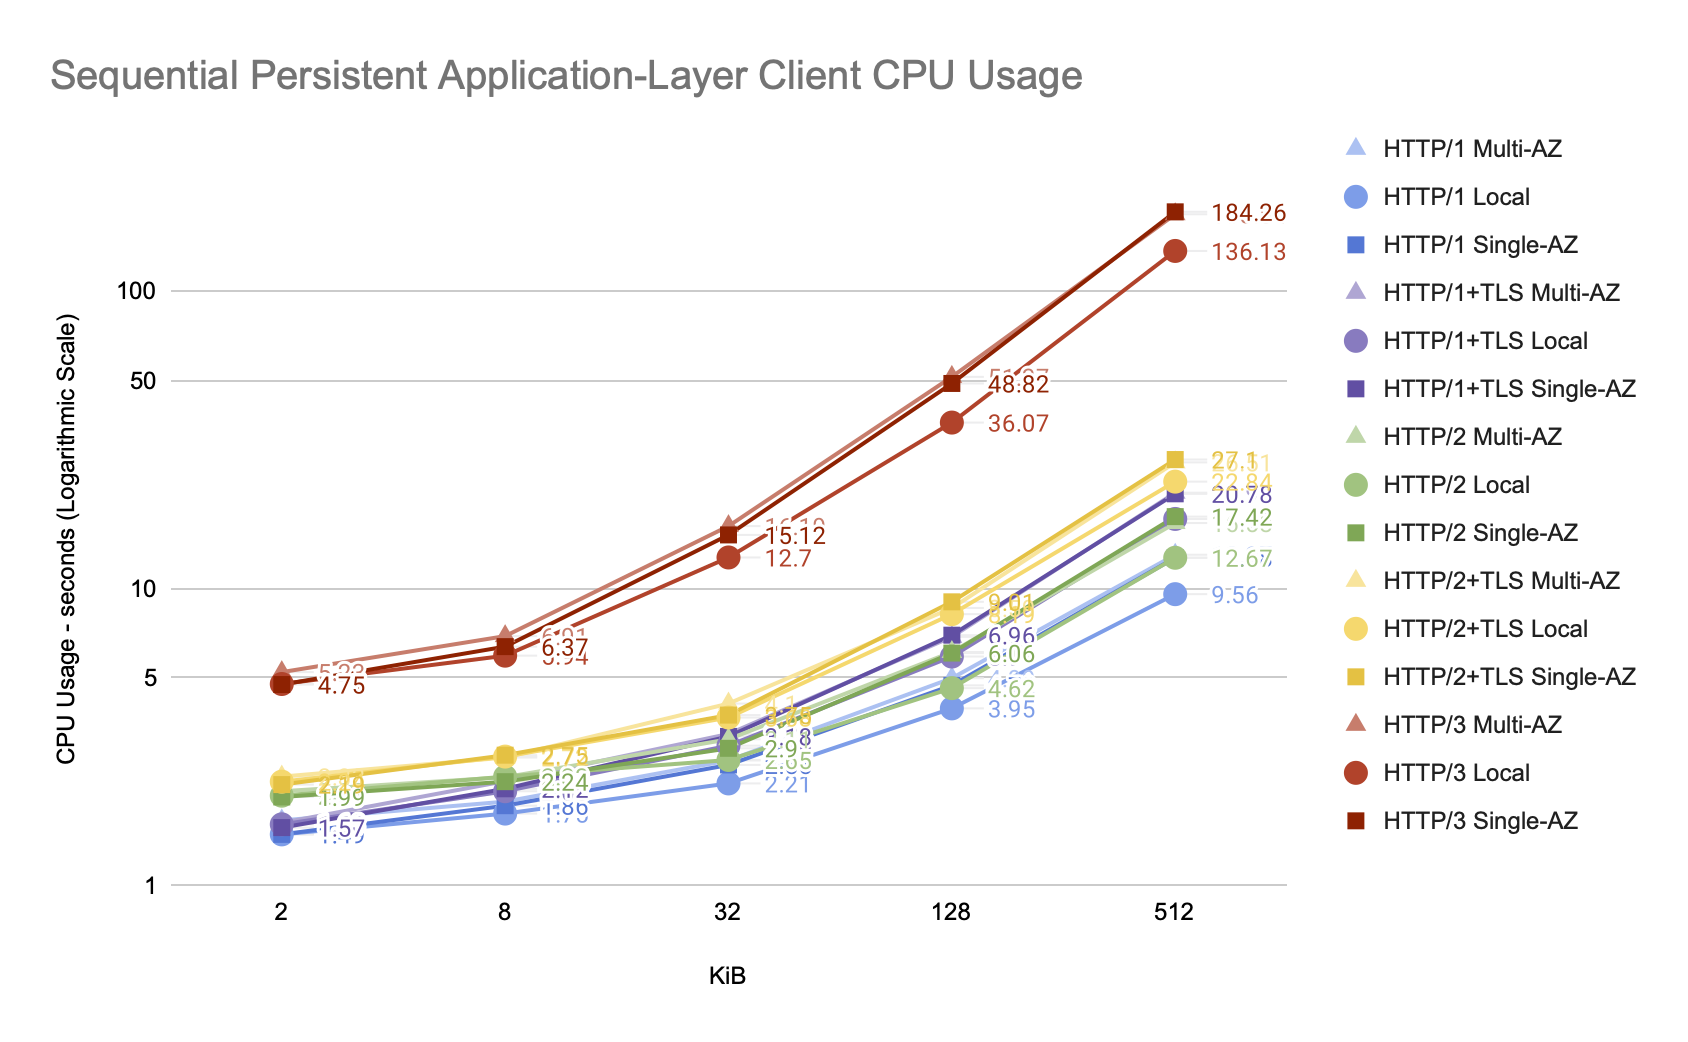
\includegraphics[width=\linewidth]{figures/charts/Sequential Persistent Application-Layer Client CPU Usage.png}
    \caption{Sequential Persistent Application-Layer Client CPU Usage}
    \label{fig:sequential_client_app_cpu}
\end{figure}
\begin{figure}[h!]
    \centering
    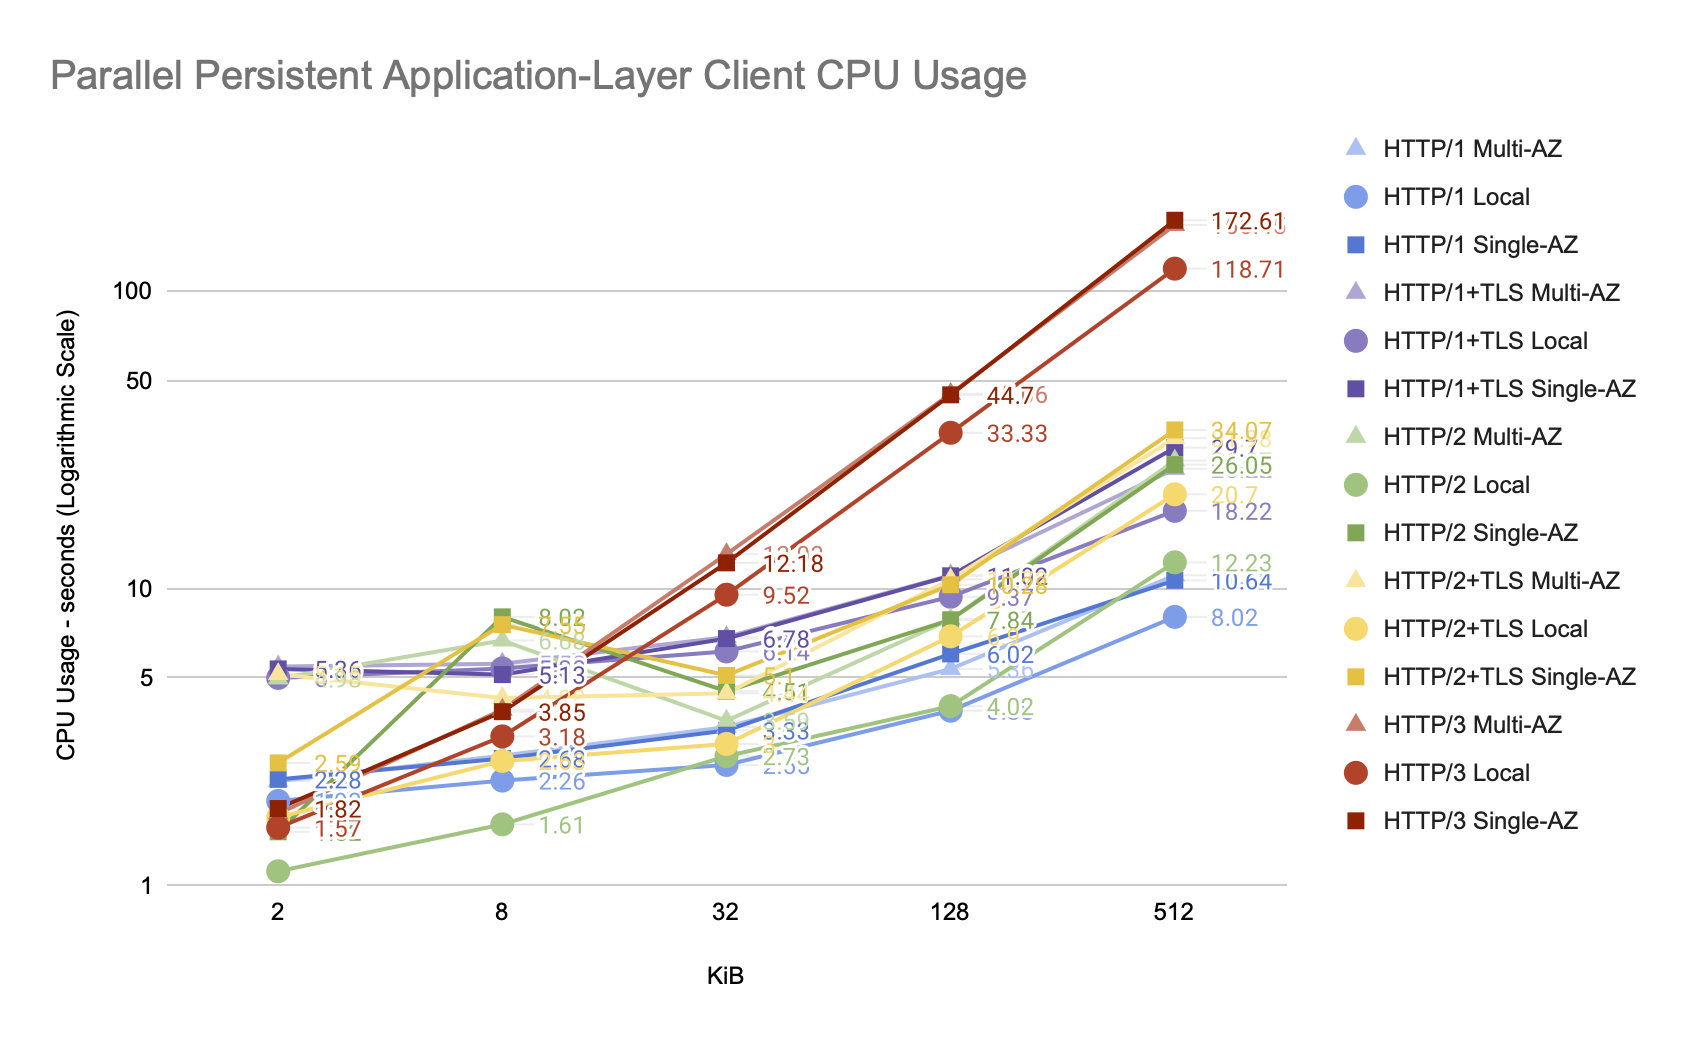
\includegraphics[width=\linewidth]{figures/charts/Parallel Persistent Application-Layer Client CPU Usage.png}
    \caption{Parallel Persistent Application-Layer Client CPU Usage}
    \label{fig:parallel_client_app_cpu}
\end{figure}

\begin{figure}[h!]
    \centering
    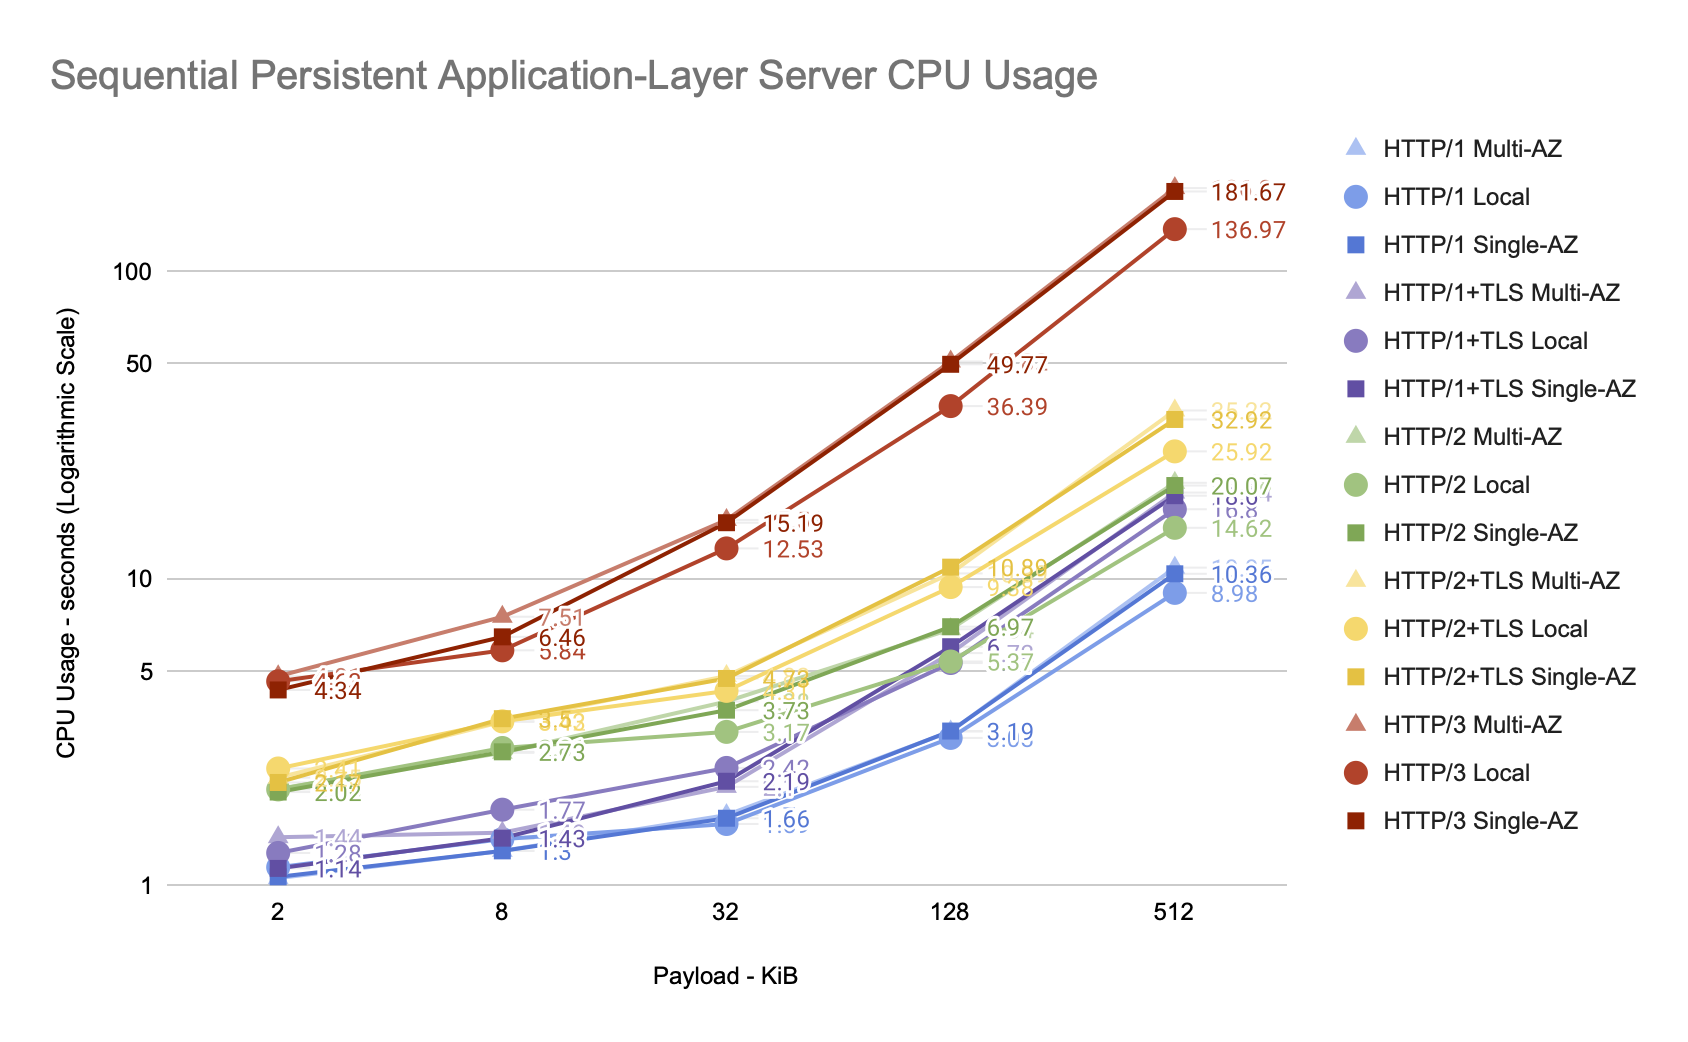
\includegraphics[width=\linewidth]{figures/charts/Sequential Persistent Application-Layer Server CPU Usage.png}
    \caption{Sequential Persistent Application-Layer Server CPU Usage}
    \label{fig:sequential_server_app_cpu}
\end{figure}
\begin{figure}[h!]
    \centering
    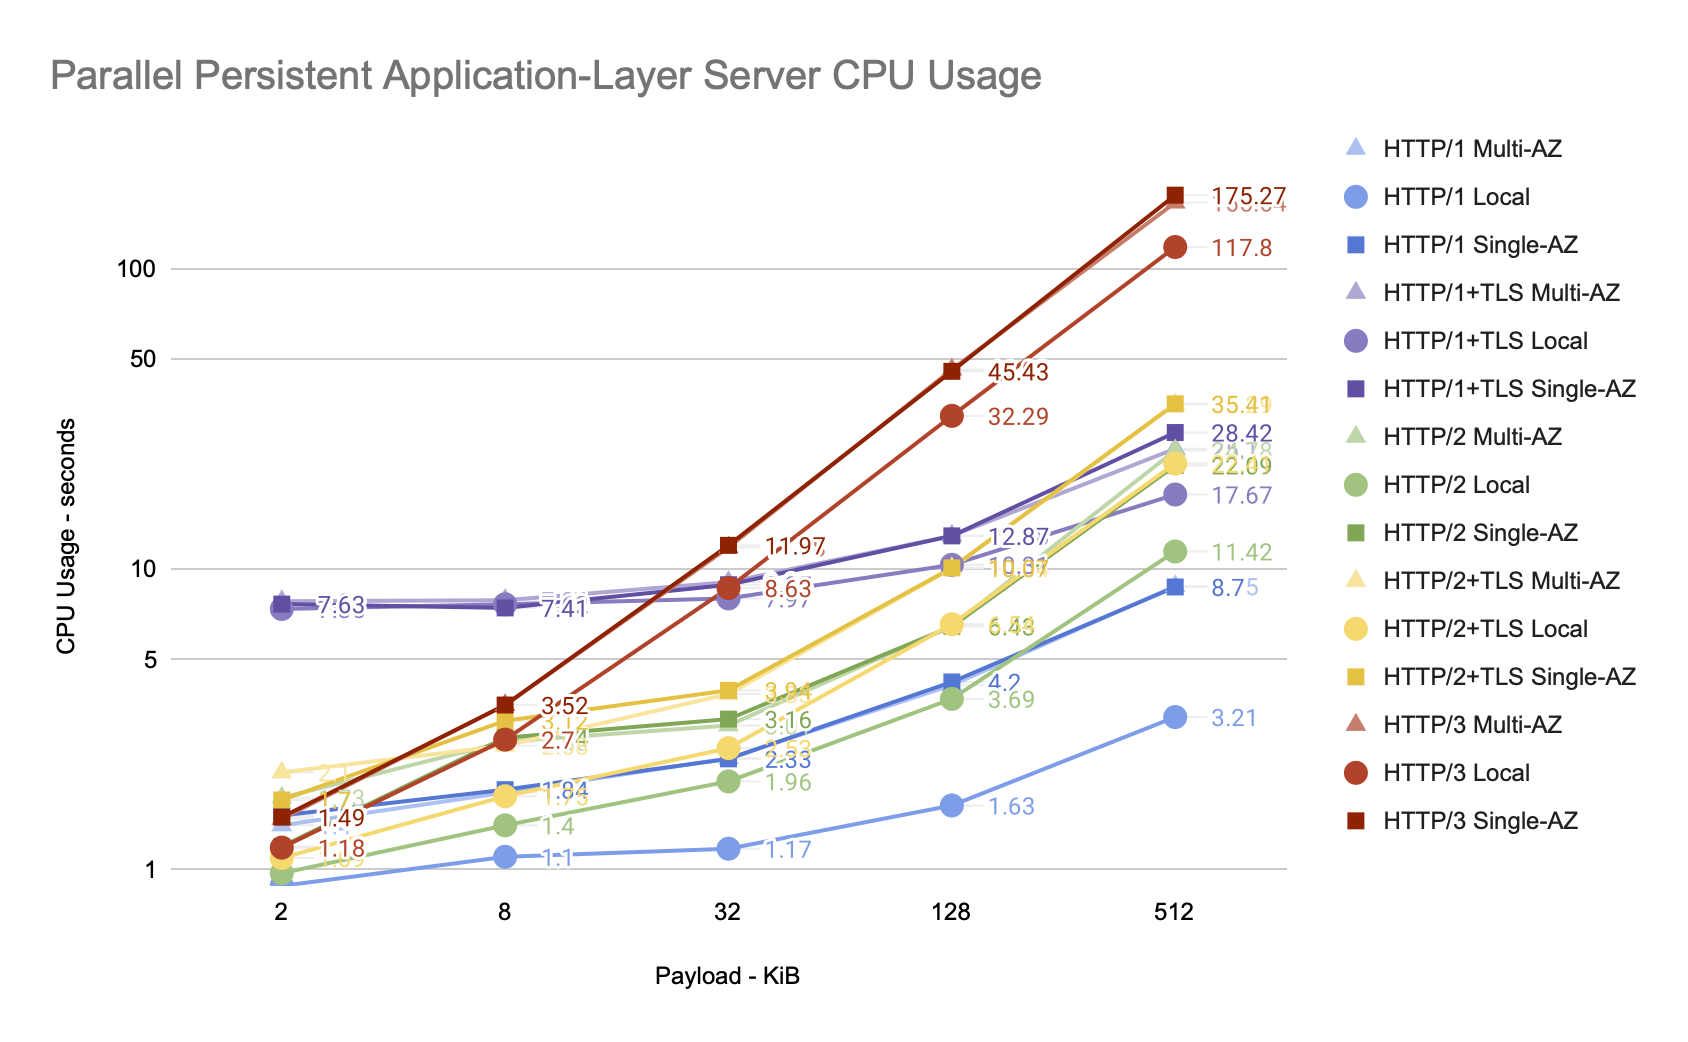
\includegraphics[width=\linewidth]{figures/charts/Parallel Persistent Application-Layer Server CPU Usage.png}
    \caption{Parallel Persistent Application-Layer Server CPU Usage}
    \label{fig:parallel_server_app_cpu}
\end{figure}
